\chapter{Machine Language Monitor}

\section{Introduction}

The machine language monitor is a debugging tool for machine language
programs. It includes a mini-assembler, a disassembler and many useful commands.
When the program execution encounters the code 00 (zero) alias BRK,
the default action of the operating system is, to call the monitor.
This features allows the debugging of programs by setting breakpoints.

\section{Table of monitor commands}

{
\ttfamily
\setlength{\tabcolsep}{1mm}
\begin{tabular}{|l|l|l|}
\hline
C & mnemonic & description \\
\hline
A &     ASSEMBLE        & Assemble a line of 45GS02 code\\
B &     BITMAPS         & Display 8x8 bitmaps (characters)\\
C &     COMPARE         & Compare two sections of memory\\
D &     DISASSEMBLE     & Disassemble a line of 45GS02 code\\
F &     FILL            & Fill a section of memory with a value \\
G &     GO              & Start execution at specified address\\
H &     HUNT            & Find specified data in a section of memory\\
L &     LOAD            & Load a file from disk\\
M &     MEMORY          & Dump a section of memory\\
R &     REGISTERS       & Display the contents of the 45GS02 registers\\
S &     SAVE            & Save a section of memory to a disk file\\
T &     TRANSFER        & Transfer memory to another location\\
V &     VERIFY          & Compare a section of memory with a disk file\\
X &     EXIT            & Exit Monitor mode\\
\hline
 . &     <period>        & Assembles a line of 45GS02 code\\
 > &     <greater>       & Modifies memory\\
 ; &     <semicolon>     & Modifies register contents\\
 @ &     <at sign>       & Disk command, directory or status\\
\hline
\$ &     <hex>           & Display hex, decimal, octal, and binary value \\
 + &     <decimal>       & Display hex, decimal, octal, and binary value\\
\& &     <octal>         & Display hex, decimal, octal, and binary value\\
\% &     <binary>        & Display hex, decimal, octal, and binary value\\
\hline
\end{tabular}
}

\section {calling the monitor}

To enter the monitor from BASIC, type:
\screentext{MONITOR}

The monitor responds with a display of register contents and waits for a command:

\begin{tcolorbox}[colback=blue,coltext=white]
\verbatimfont{\codefont}
\begin{verbatim}
MONITOR
\end{verbatim}
\begin{tcolorbox}[colback=yellow,coltext=blue,,arc=0mm,boxrule=0mm,
       left*=0.5mm,right*=0mm,top=0mm,bottom=0mm,nobeforeafter,
       left skip=0.1mm,
       width=50mm,height=3mm,valign=center]
\begin{verbatim}
BS MONITOR COMMANDS:ABCDFGHJMRTX@.>;?$+&%'LSV
\end{verbatim}
\end{tcolorbox}
\begin{verbatim}
    PC   SR AC XR YR ZR BP  SP  NVEBDIZC
; 00CFA4 35 00 00 00 00 00 01F8 --11-1-1
\end{verbatim}
\end{tcolorbox}

% ======================================
% Start of the monitor command reference
% ======================================

\titleformat*{\subsection}{\normalfont\huge\bfseries\color{blue}}

% ***********
% DISASSEMBLE
% ***********

\subsection{D : DISASSEMBLE}
\index{DISASSEMBLE}
\index{MONITOR Commands!DISASSEMBLE}
\begin{description}[leftmargin=2cm,style=nextline]
\item [Format:] {\bf D [from [,to]]}
\item [Usage:] Prints a machine language listing for the specified
               address range assuming, that it contains code.
               If only one argument is present, the disassembler
               disassembles the next 21 bytes. If no argument is
               given, the disassembly continues with the last used
               disassemble address.
               The contents are printed as hex values.

\item [Remarks:] The rows start with the dot character '.'.
                 This enables direct full screen editing of the disassembly.
                 Typing return in any row will assemble the changed
                 command of the cursor row back to memory, if writable RAM is there.
                 See monitor command {\bf .}.

                 The disassembler knows the instruction set of the C65 CPU
                 GS6502. Enhanced instructions from the 45GS02 CPU of the MEGA65
                 are not recognised.

\item [Example:] Using {\bf D}
\end{description}

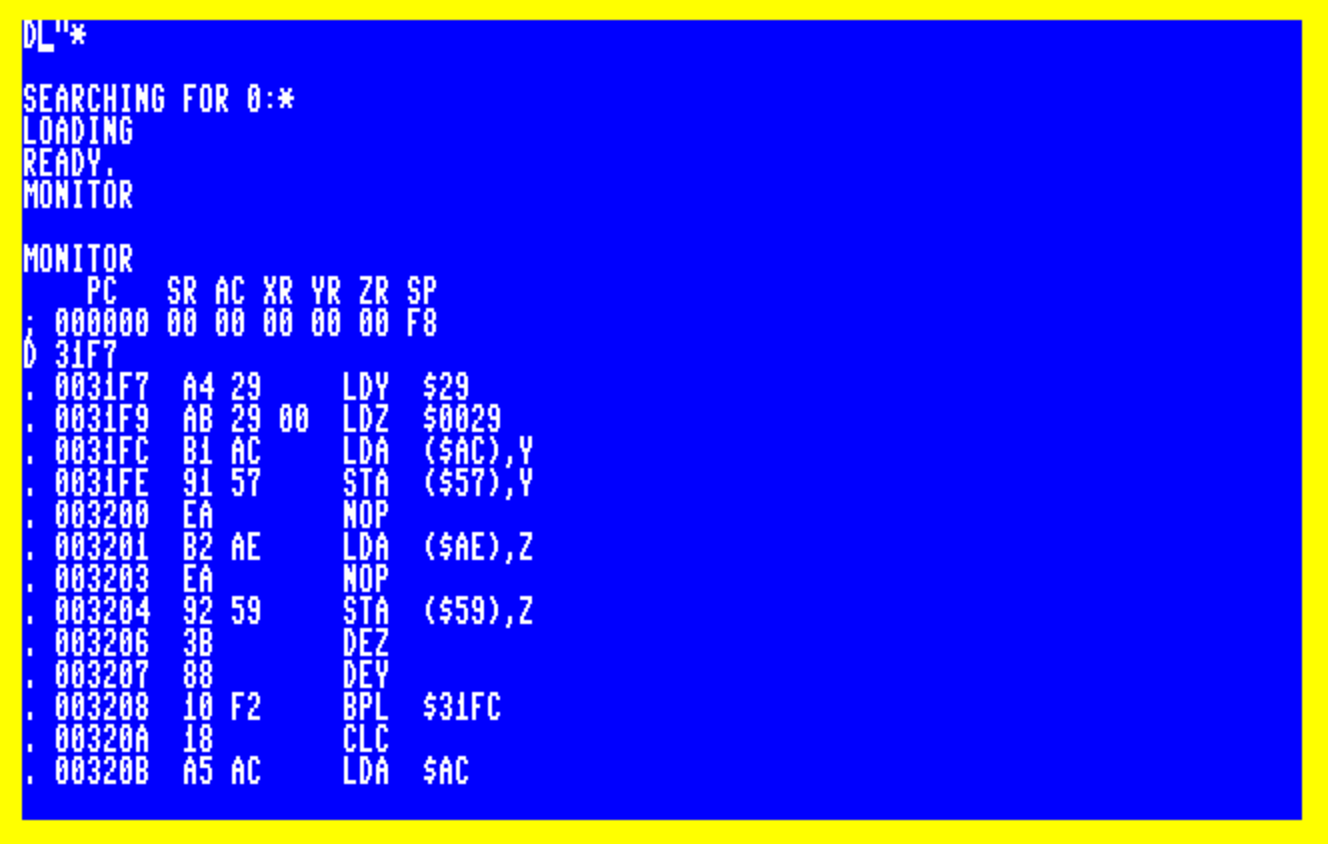
\includegraphics[width=\linewidth]{images/monitor-d}

% ******
% MEMORY
% ******

\subsection{M : MEMORY}
\index{MEMORY}
\index{MONITOR Commands!MEMORY}
\begin{description}[leftmargin=2cm,style=nextline]
\item [Format:] {\bf M [from [,to]]}
\item [Usage:] Prints a memory dump for the given address range.
               The dump displays memory contents, organized in rows
               of 16 consecutive addresses starting with the
               address, given as 1st. argument. The dump continues
               until a row has been printed, containing the value
               of the address given as 2nd. argument.
               If no 2nd. argument is present, the dump displays
               a full page of 256 bytes in 16 rows.
               The contents are printed as 16 byte values in hex,
               followed by the character representation.

\item [Remarks:] The rows start with the character '>'.
                 This enables direct full screen editing of the dump.
                 Typing return in any row will write the changed
                 values of the cursor row back to memory, if writable RAM is there.
                 See monitor command {\bf >}.

\item [Example:] Using {\bf M}
\end{description}

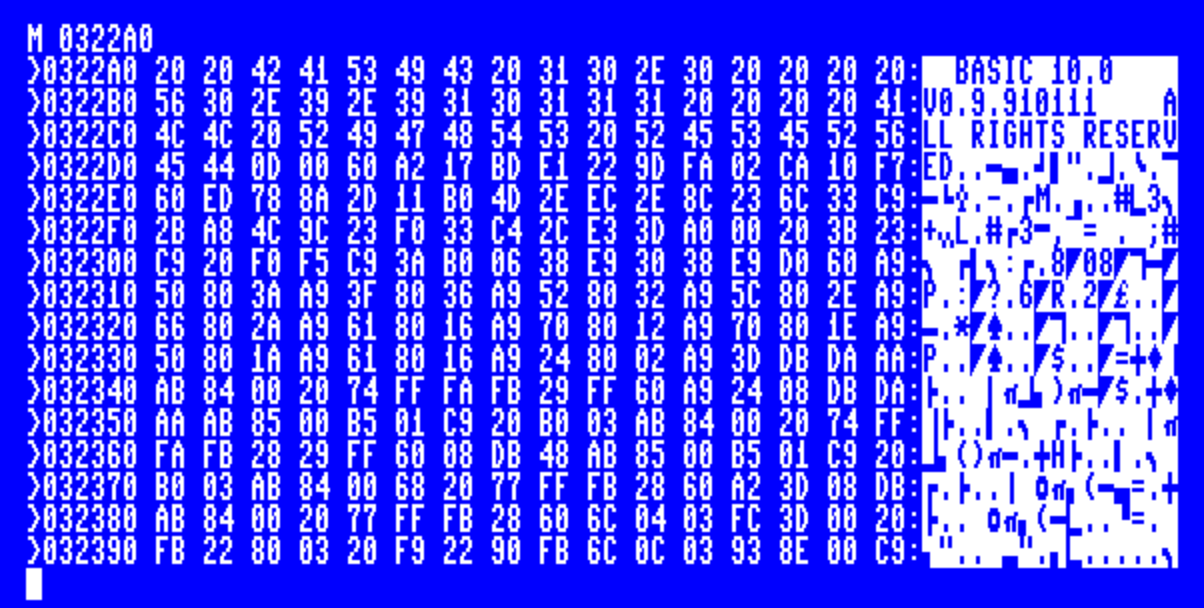
\includegraphics[width=\linewidth]{images/monitor-m}

